\subsubsection{Representaci\'on con compuertas AND, OR y NOT}
\noindent
La representaci\'on de la expresion obtenida previamente mediante compuertas logicas AND, OR y NOT se puede ver a continuaci\'on, en la figura \ref{fig:ej2b}

\begin{figure}[H]
    \centering
    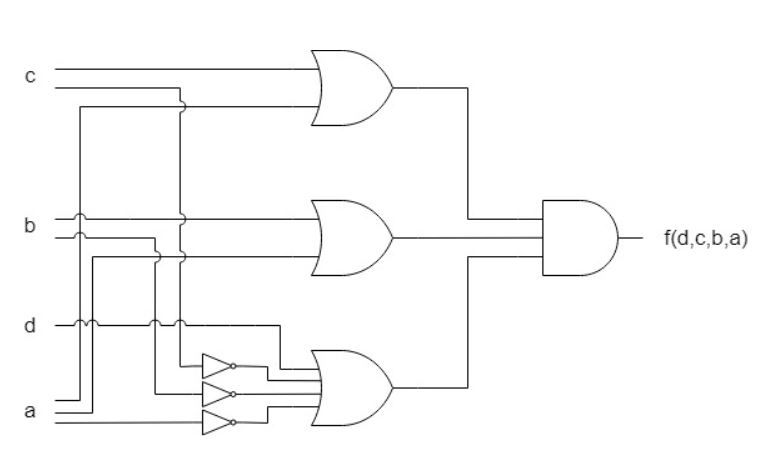
\includegraphics[scale=0.55]{images/ej2/circuito1_ej2_parteb.JPG}
    \caption{Circuito con compuertas AND, OR y NOT}
    \label{fig:ej2b}
\end{figure}

\subsubsection{Representaci\'on con compuertas NAND}
\noindent
La representaci\'on de la expresi\'on obtenida previamente mediante compuertas logicas NAND se puede ver a continuaci\'on en la figura \ref{fig:ej2bnand}

\begin{figure}[H]
    \centering
    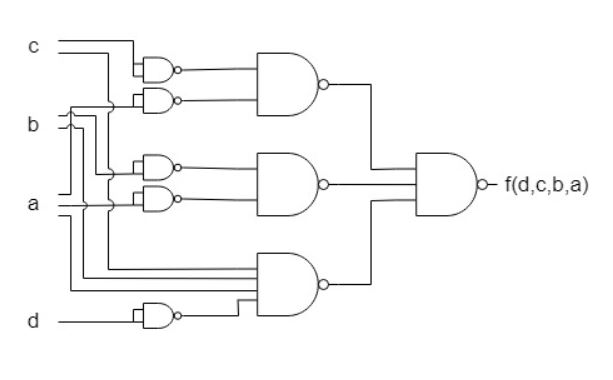
\includegraphics[scale=0.7]{images/ej2/circuito2_ej2_parteb.JPG}
    \caption{Circuito con compuertas NAND}
    \label{fig:ej2bnand}
\end{figure}\\